%%%%%%%%%%%%%%%%%%%%%%%%%%%%%%%%%%%%%%%%%%%%%%%%%%%%%%%%%%%%%%%%%%%%%%
% 
% This .tex file is coded in utf-8
% 
%%%%%%%%%%%%%%%%%%%%%%%%%%%%%%%%%%%%%%%%%%%%%%%%%%%%%%%%%%%%%%%%%%%%%%
\chapter{分析力学}
\section{变分法与Euler-Lagrange方程}

%含目标的优化,给出所求解的函数是很重要的问题。
%求函数的极值与求泛函的极值$\leftrightarrow\aleph_1$ 与 $\aleph_2$

如何寻找极值函数?

\subsection{最速降线}

问题:如何用一条光滑的滑轨连接A,B两点,使得某个小球沿此光滑轨道从A到B时间最短。如图:

\begin{figure}[htbp!]
	\centering
	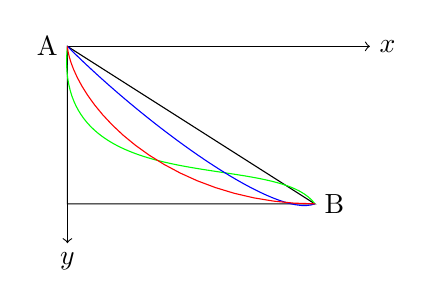
\begin{tikzpicture}
		\node[above,left](A) at (0,0) {A};
		\node[below,right](B) at (pi,-2){B};
		\node[right](x) at (pi + 0.7,0){$x$};
		\node[below](y) at (0,-2-0.5){$y$};
		\draw[->] (0,0) -- (pi + 0.7,0);
		\draw[->] (0,0) --(0,-2-0.5);
		\draw (0,0) -- (0,-2) -- (pi,-2) -- cycle;
		\draw[green] (0,0) .. controls (-0.2,-2) and (pi-0.5,-1.3)  .. (pi,-2);
		\draw[blue] (0,0) .. controls (1,-1) and (pi-0.5,-2.2)  .. (pi,-2);
		\draw[red] plot[domain=0:pi] ({\x - sin(\x r)},{-1 + cos(\x r)});
	\end{tikzpicture}
	\caption{哪个是最速降线?}
\end{figure}

所需总时间:
\[T = \int_{A}^{B} \mathrm{d}T = \int_{A}^{B} \frac{\mathrm{d}L}{v} = \int_{A}^{B} \frac{\sqrt{\mathrm{d}x^2+\mathrm{d}y^2}}{\sqrt{2gy}} = \int_{A}^{B} \frac{\sqrt{1+y'^2}}{\sqrt{2gy}}\mathrm{d}x\]
抽象$\Rightarrow$:
\begin{equation}
S = \int L(f(x),f'(x),x)\mathrm{d}x
\end{equation}
待求函数$f(x)$,使得$S$取极值。数学上这种函数叫做泛函。

\subsection{Euler-Lagrange方程}
求以下泛函的极值:
\begin{equation}
S = \int_{x_1}^{x_2} L(f(x),f'(x))\mathrm{d}x
\end{equation}
函数极值问题启示我们应该在极值函数上尝试做微小改变。

目标极值函数$f_0(x)$,微小改变$|\delta(x)|\ll1$,其中微小改变$\delta(x) = \epsilon \eta(x),\epsilon\rightarrow0$且$\eta(x)$为任意函数。又在端点处应满足:$\delta(x_1) = \delta(x_2) = 0$,所以$\eta(x_1) = \eta (x_2) = 0$,此时有:
\begin{equation}
S = \int_{x_1}^{x_2}L(f,f')\mathrm{d}x \ge S' = \int_{x_1}^{x_2}L(f+\epsilon\eta,f'+\epsilon\eta')\mathrm{d}x
\end{equation}
可将$S$看作$\epsilon$的函数$S(\epsilon)$,在$\epsilon=0$时取极值。即:
\begin{align*}
S'(\epsilon) &= 0\\
             &= \int_{x_1}^{x_2} \left[ \frac{\partial L}{\partial(f+\epsilon\eta)} \cdot \frac{\partial(f+\epsilon\eta)}{\partial\epsilon} + \frac{\partial L}{\partial(f'+\epsilon\eta')} \cdot \frac{\partial(f'+\epsilon\eta')}{\epsilon} \right] \mathrm{d}x\\
             &= \int_{x_1}^{x_2} \left( \frac{\partial L}{\partial f} \cdot \eta + \frac{\partial L}{\partial f'} \cdot \eta' \right)\mathrm{d}x\\
             &= \int_{x_1}^{x_2}  \frac{\partial L}{\partial f} \cdot \eta \mathrm{d}x + \left. \frac{\partial L}{f'} \cdot \eta \right|_{x_1}^{x_2} - \int_{x_1}^{x_2} \left(\frac{\partial L}{f'}\right)'\cdot \eta \mathrm{d}x\\
             &= \int_{x_1}^{x_2} \left[ \frac{\partial L}{\partial f} - \left(\frac{\partial L}{\partial f'}\right)' \right] \cdot \eta \mathrm{d}x = 0
\end{align*}
因为$\eta(x)$是任意函数,所以:
\begin{equation}
\frac{\partial L}{\partial f} - \frac{\mathrm{d}}{\mathrm{d}x}\left(\frac{\partial L}{\partial f'}\right) = 0
\end{equation}
此即Euler-Lagrange方程。

\[S = \int L \mathrm{d}t\]
$S$:作用量(Action),$L$:拉格朗日量(Lagrangian)

!!!!!为何要求在端点处应满足:$\delta(x_1) = \delta(x_2) = 0$,即$\eta(x_1) = \eta (x_2) = 0$!!!!!

\subsection{路径积分的权重因子}

粒子从A到B有多个路径,对每个路径有相应的作用量$S$,每个作用量赋予其一个权重因子:
\[e^{i\frac{S}{\hbar}}\]
对所有路径求和:
\[\sum_{\text{所有路径}}e^{i\frac{S}{\hbar}}\]
此即路径积分因子。<态和态之间的投影因子。>

\subsection{E-L方程应用举例}

\begin{enumerate}
	\item 
		证明:两点间直线最短。
		
		证明:任意两点间距离:
		\[\Delta L^2 = \Delta x^2 + \Delta y^2\]
		作用量为:
		\[S = \int_{A}^{B} \mathrm{d}L = \int_{A}^{B} \sqrt{\mathrm{d}x^2+\mathrm{d}y^2} = \int_{x_A}^{x_B} \sqrt{1 + y'^2} \mathrm{d}x\]
		代入E-L方程:
		\[\frac{\mathrm{d}}{\mathrm{d}x} \left( \frac{\partial \sqrt{1 + y'^2}}{\partial y'} \right) = 0\]
		所以:
		\[\frac{y'}{\sqrt{1 + y'^2}} = C_1 \]
		即:
		\[y' = constant\]
		此即两点间直线最短。\\
	\item
		最小用料问题:优化圆台的侧面使得其侧面面积最小。如图。
		\begin{figure}
			\centering
			\subfigure{\includegraphics[width=6cm]{Figures/chimney.pdf}}
			\subfigure{\includegraphics[width=4.7cm]{Figures/chimneysol.pdf}}
			\caption{最小用料问题}
		\end{figure}
		其作用量为:
		\[S = \int_{r_1}^{r_2} 2\pi \sqrt{1+y'^2}\mathrm{d}x\]
		代入E-L方程可得:
		\[\frac{\mathrm{d}}{\mathrm{d}x} \left( \frac{2\pi x y'}{\sqrt{1+y'^2}} \right) = 0\]
		所以:
		\[\frac{x y'}{\sqrt{1+y'^2}} = C_1\]
		即:
		\[y' = \frac{C_1}{\sqrt{x^2-C_1^2}}\]
		所以可以解得:
		\begin{equation}
		\left\{
		\begin{array}{c}
		y = \mathrm{arccosh} \frac{x}{C_1} + C_2\\
		x= C_1 \cosh (y-C_2) 
		\end{array}
		\right.
		\end{equation}
		
		由端点可以确定$C_1,C_2$。
	\item
		给定$z^2 = 8(x^2+y^2)$求连接其上任意两点A,B的曲线方程。
		
		解:采用柱坐标$(z,r,\theta)$,曲面方程变为:$z=8r^2$,曲面上微元的长度:
		\[\mathrm{d}l^2 = 9\mathrm{d}r^2+r^2\mathrm{d}\theta^2\]
		曲线长度:
		\[L = \int_{A}^{B} \mathrm{d}L = \int_{A}^{B}\sqrt{9\mathrm{d}r^2+r^2\mathrm{d}\theta^2} = \int_{A}^{B}\sqrt{9+r^2\theta'^2}\mathrm{d}r\]
		代入E-L方程:
		\[\frac{\mathrm{d}}{\mathrm{d}\theta}\left( \frac{\partial L}{\partial \theta'} \right) = \frac{\mathrm{d}}{\mathrm{d}\theta}\left( \frac{r^2\theta'}{\sqrt{9+r^2\theta'^2}} \right) =0\]
		所以:
		\[\frac{r^2\theta'}{\sqrt{9+r^2\theta'^2}} = k\]
		所以:
		\[\theta' = \frac{3k}{r\sqrt{r^2-k^2}}\]
		所以:
		\begin{equation}
		\left\{
		\begin{array}{c}
		r\cos \left(\frac{\theta+\alpha}{3}\right) = k\\
		z = 2\sqrt{2}r
		\end{array}
		\right.
		\end{equation}
		其中$\alpha,k$为待定常数。
\end{enumerate}

\subsection{理论力学框架}

\begin{tikzpicture}
	\node[above](A) at (0,0) {极值问题};
	\node[below,left](B) at (-1,-1){E-L方程} ;
	\node[below,right](C) at (1,-1) {牛顿力学,量子力学...};
	\draw[<->] (A) -- (B);
	\draw[<->] (B) -- (C);
	\draw[<->] (C) -- (A);
\end{tikzpicture}

\subsubsection{改造牛顿第二定律}